% ============================================================
% 3. System Architecture & Implementation (~800 words)
% ============================================================
\section{System Architecture \& Implementation}
\label{sec:architecture}

This section details the system architecture, infrastructure deployment, and technical implementation of our robust data pipeline. We outline the hardware topology deployed on OpenStack, why we selected our core software stack, and the engineering mechanisms driving our ETL and analysis jobs. 

% --- 3.1 System Design ---
\subsection{System Design}
\label{subsec:system-design}

Our system follows a classic centralized-master, distributed-worker model tailored for batch processing big data. As depicted in Figure~\ref{fig:architecture}, the architecture is divided into three primary layers: Ingestion, Distributed Storage (HDFS), and Distributed Processing (Apache Spark). Data is fetched externally into the master node, pushed to HDFS, and subsequently processed by Spark executors dispersed across the worker nodes.

\begin{figure}[H]
    \centering
    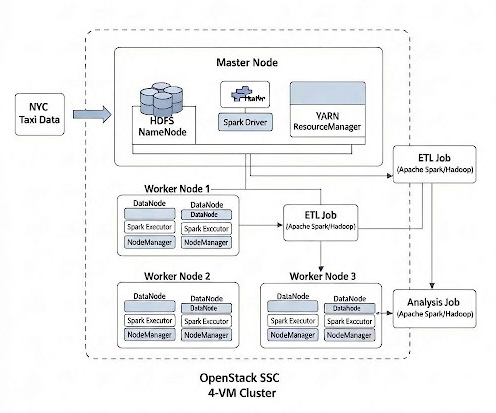
\includegraphics[width=0.85\textwidth]{figures/cluster-architecture.jpg}
    \caption{System architecture diagram showing the OpenStack deployment, node topology, and the internal data pipeline flow from raw Parquet to aggregated results.}
    \label{fig:architecture}
\end{figure}

% --- 3.2 Technology Stack ---
\subsection{Technology Stack}
\label{subsec:tech-stack}

Given the project requirements, we adopted a modern big data stack focused on in-memory processing capabilities:
\begin{itemize}
    \item \textbf{Storage (HDFS via Hadoop 3.4.1)}: Chosen for its fault tolerance and native integration with Spark. While cloud object storage (like AWS S3) is popular today, deploying HDFS on bare VMs offers direct control over data locality and block replication factors.
    \item \textbf{Processing (Apache Spark \& PySpark 3.5.1)}: We selected Spark over standard Hadoop MapReduce because Spark holds intermediate RDDs and DataFrames in memory, drastically accelerating the iterative transformations required during our ETL phase. PySpark provides an accessible DataFrame API and straightforward type-casting structures.
    \item \textbf{Orchestration \& Resource Management}: We relied on standalone cluster management managed heavily by Bash scripts (\texttt{run\_benchmark.sh} and \texttt{deploy.sh}) combined with Git for CI/CD, creating a lightweight yet effective pipeline orchestration.
\end{itemize}

% --- 3.3 Infrastructure Configuration ---
\subsection{Infrastructure Configuration}
\label{subsec:infra}

Our cluster is deployed entirely on the Swedish National Infrastructure for Computing (SNIC) OpenStack instance. The infrastructure consists of 4 tightly coupled Virtual Machines (VMs):
\begin{itemize}
    \item \textbf{Master Node (1x ssc.medium)}: 2 vCPU, 4 GB RAM. This node is assigned a Floating IP for external SSH access. It houses the Hadoop NameNode, ResourceManager, and the Spark Driver process.
    \item \textbf{Worker Nodes (3x ssc.medium)}: 2 vCPU, 4 GB RAM each. These sit on a private sub-network (192.168.2.x subnet). They run the Hadoop DataNodes, NodeManagers, and Spark Executor instances.
\end{itemize}
In total, the cluster harnesses 8 vCPUs and 16 GB of RAM, capped with a strict 100 GB collective storage limit. To maintain data reliability without exceeding storage quotas, HDFS was configured with a replica factor of 2 (\texttt{dfs.replication=2}). 

% --- 3.4 Data Pipeline ---
\subsection{Data Pipeline}
\label{subsec:pipeline}

The pipeline executes in three synchronized stages:
\begin{enumerate}
    \item \textbf{Ingestion}: Raw NYC Taxi Parquet files are downloaded from the TLC portal to the Master node via \texttt{wget} and deposited straight into \texttt{hdfs://.../data/nyc-taxi/}.
    \item \textbf{ETL Phase}: The \texttt{etl\_job.py} script ingests the raw data block by block. It filters out invalid records (e.g., zero-distance trips, null metrics), converts timestamps to calculate \texttt{duration\_minutes} and \texttt{pickup\_hour}, aggressively prunes dropped columns, and commits the clean records back to HDFS at \texttt{/data/nyc-taxi-cleaned/}.
    \item \textbf{Analysis Phase}: Finally, \texttt{analysis\_job.py} aggregates the validated dataset. It groups by \texttt{PULocationID} and \texttt{pickup\_hour} to compute the average fare and trip duration. It subsequently performs a left join against a static CSV (\texttt{taxi\_zone\_lookup.csv}) to convert abstract ID numbers into human-readable zone names, coalescing the final output into a single file for stakeholder ingestion.
\end{enumerate}

% --- 3.5 Code Structure ---
\subsection{Code Structure}
\label{subsec:code-structure}

The codebase follows a modular design paradigm:
\begin{itemize}
    \item \textbf{\texttt{src/config.py}}: Centralizes cluster endpoints, absolute HDFS URI paths, and basic threshold configurations to eliminate hardcoded parameters across jobs.
    \item \textbf{\texttt{src/etl\_job.py}}: The heaviest processor. Given resource constraints, it bypasses standard \texttt{spark.read.parquet("*.parquet")} schema inferences and iteratively targets singular files using \texttt{subprocess.run} to interact with HDFS.
    \item \textbf{\texttt{src/analysis\_job.py}}: Houses the PySpark SQL aggregations, strictly outputting to a targeted CSV path using \texttt{coalesce(1)}.
    \item \textbf{\texttt{scripts/run\_benchmark.sh}}: A specialized harness that automates execution over varied core allocations (\texttt{--total-executor-cores}) and node arrays to capture timestamps for plotting horizontal and vertical scales.
\end{itemize}

% --- 3.6 Challenges & Solutions ---
\subsection{Challenges \& Solutions}
\label{subsec:challenges}

We encountered several prominent technical challenges during development:
\begin{enumerate}
    \item \textbf{Dataset Schema Volatility}: When reading multi-month TLC data, PySpark's vectorized Parquet reader routinely crashed (\texttt{[CANNOT\_MERGE\_SCHEMAS]}) due to invisible shifts in the column type for \texttt{Airport\_fee} (varying from \texttt{INT32} to \texttt{FLOAT64} dynamically by month). 
    \textit{Solution}: We restructured the ETL job into a \texttt{for}-loop that asks HDFS for the explicit list of file paths. Spark reads them independently, safely infers local schemas, selectively prunes the offensive column, and appends into a normalized structure.
    \item \textbf{Strict Storage Exhaustion}: 25 GB of storage per VM meant HDFS was easily overwhelmed caching uncompressed RDDs and saving multiple layers of Parquet processing data.
    \textit{Solution}: We established an aggressive "select and drop" mechanism in the ETL. We discard roughly 15 unused columns representing several gigabytes of overhead, saving only the 4 tightly packed elements (\texttt{PULocationID}, \texttt{fare\_amount}, \texttt{pickup\_hour}, \texttt{duration\_minutes}) needed for analysis.
    \item \textbf{Dynamic Allocation Skewing Benchmark Constraints}: Spark's dynamic resource allocation skewed the early iterations of our benchmarking by automatically distributing workloads across nodes we were attempting to restrict. 
    \textit{Solution}: We disabled dynamic allocation directly via PySpark config keys (\texttt{spark.dynamicAllocation.enabled=false}) and enforced hard caps using Spark submit metrics.
\end{enumerate}
